\chapter{Introduction}
\label{ch:introduction}
\glsresetall

\section{Problem Background}
\label{ch:problem_statement}

The Department of Defense Electromagnetic Spectrum Superiority Strategy states clearly that the Electromagnetic spectrum is a battleground, inseparable from the classical settings of war. The expectation for future near-peer conflict will result in a highly `congested, contested, and constrained Electromagnetic Operating Environment (EMOE) \cite{DOD_ESSS}' The DoD EMSSS seeks to develop equipment that will be flexible, efficient, resilient. This project seeks to support this vision for the future EMS war by examining tactics that create congestion and confusion in the EMOE. Particularly, the employment of air borne platforms.

Decoy airborne platforms were conceptualized as early as 1952, with the development and test of the XSM-73 `Goose' ground-launched airborne decoy which was later reconfigured as an air-launched platform, and re-designated the ADM-20 `Quail'. The Quails' purpose was to overwhelm an adversary integrated air-defense system (IADS), allowing for bomber and strike aircraft to penetrate the airspace and prosecute targets. The Quail was succeeded by the ADM-141 TALD, or Tactical Air-Launch Decoy which was employed with good effect during the first night of the Gulf War. Launched in coordination with BQM-74 target drones, the decoy platforms were launched towards Baghdad to force a response from adversary IADS. The operation was a success:  adversary radars were forced to engage the unknown targets, which opened them up to attack from Coalition Anti-Radiation missiles. There was an additional benefit of forcing attrition on the Iraqi Air Defense's Surface to Air missile stores:  the cheaply produced decoys were an effective sponge for the more costly surface to air missiles.

Airborne decoys play a specific role in the contested EMOE:  they degrade the air defenders view of the scene; force radars to engage the decoys, exposing themselves to anti-radiation fires; and force engagement, which depletes the IADS available surface to air missile stores.

The power of decoy missiles is that on physical inspection they appear similar in shape size, and speed to their lethal relatives. An example is shown in figure \ref{fig:missiles}, where an air-launched decoy is set alongside its potentially nuclear-equipped cousin.

\begin{figure}[htbp]
  \centering
  \begin{subfigure}{.5\textwidth}
    \centering
    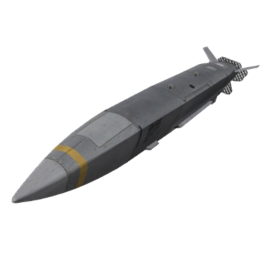
\includegraphics[width=.8\linewidth]{adm-160.png}
  \end{subfigure}%
  \begin{subfigure}{.5\textwidth}
    \centering
    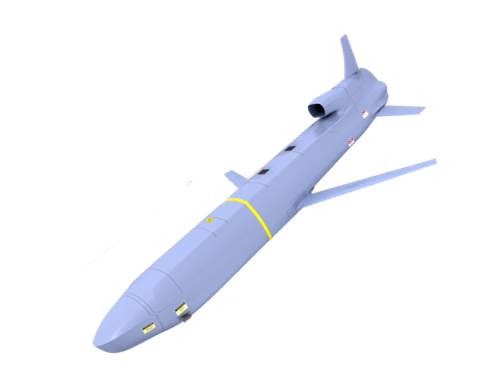
\includegraphics[width=.8\linewidth]{agm-86.png}
  \end{subfigure}
  \caption[Air Launched Platform Comparison]{An ADM-160B MALD and AGM-86 Air Launched Cruise Missile (ALCM)}
  \label{fig:missiles}
\end{figure}


This paper seeks to a solution to this problem:  a hypothetical sensor with an embedded machine learning model is trained to classify similar targets using radar cross section data. This project accepts the likelihood that the true RCS data for an adversary target would not be available, and instead utilizes simulation data to train the model. The models performance is tested using measurement data taken from an open-air range.


\section{Research Objectives}
\label{sec:objectives}

The principle goals of this project are to analyze and document the performance of a machine learning network's ability to classify targets. The model will be trained using simulation data, and evaluated using measured data. Additionally, this paper will document data normalization techniques for RCS data; quantify sensor performance breakdowns in terms of signal correlation; as well as document performance enhancing techniques such as multi-model comparators, and multi-angle training.

\section{Document Overview}
\label{sec:overview}

Chapter 2 of this document cover background information relevant to this project: radar operation, electromagnetic waves and target interaction, as well as a review of similar projects and the current state of machine learning models in signal processing. Chapter 3 will outline the methodology employed in this experiment to include data collection for both simulated and measured targets; measurement calibration; data augmentation, and model evaluation. Chapter 4 will report the experiments findings, and chapter 5 will present a conclusion
